\documentclass[a4paper,12pt]{article}
%\usepackage[latin1]{inputenc}
\usepackage[spanish]{babel}
\usepackage{graphicx}
\usepackage{amsmath}
\spanishdecimal{.}
\usepackage{wrapfig}
\setlength{\textheight}{250mm}
\setlength{\textwidth}{165mm}
\setlength{\topmargin}{-15mm}
\setlength{\oddsidemargin}{0pt}
\pagestyle{empty}


\renewcommand{\labelenumi}{\alph{enumi})}

\begin{document}

\def\bm#1{{\mbox{\boldmath $#1$}}}
\def\eqdef{\buildrel \rm def \over =}
\def\signo{\mathop{\rm signo}\nolimits}

\mbox{}\vspace*{-20mm}

{\centering
{\small\sc %Escuela Técnica Superior de Ingenieros de Caminos, Canales y Puertos (Madrid)}\\*[4mm]
Máster Universitario en Ingeniería de Estructuras, Cimentaciones y Materiales}\\*[4mm]
{\Large\bf Método de los Elementos Finitos 23-24}\\*[4mm]
PRÁCTICA 4: Elasticidad lineal (elementos 2D). \\*[4mm]}

% \vspace{4mm}

% ENUNCIADO
\begin{wrapfigure}[18]{r}[5mm]{70mm}
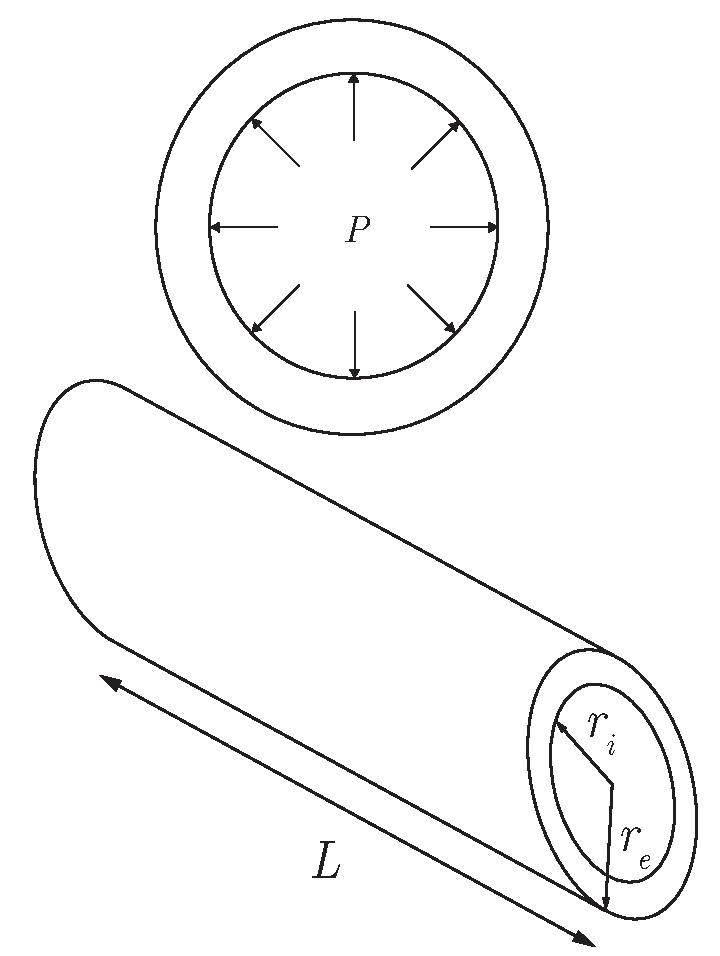
\includegraphics[width=70mm]{cargas}
\end{wrapfigure}

En esta práctica se analiza un tubo de sección circular, longitud indefinida, $L$, y sometido a presión interna, empleando para ello un modelo de deformación plana.\\

Los valores de los distintos parámetros que definen el problema son:

\begin{itemize}
\item  \texttt {$r_i$}: Radio interior del tubo = 0.5 m.
\item \texttt {$r_e$}: Radio exterior del tubo = 1.0 m.
\item \texttt {$P$}: Presión interna = 300 MPa.
\item \texttt {$E$}: Módulo de Young = 2.1 $\cdot10^5$ MPa.
\item \texttt {$\nu$}: Coeficiente de Poisson 0.3.
\end{itemize}

La malla estará formada por elementos cuadriláteros lineales (CPE4) para deformación plana con tamaño aproximado de 0.1 m. Posteriormente, se realizará el cálculo utilizando esta vez cuadriláteros cuadráticos (CPE8). Se comprobarán los resultados obtenidos en tensiones y desplazamientos con la solución teórica.\\

Se pide medir la fuerza circunferencial que se ejerce en el tubo con elementos CPE8 (comprobar que da alrededor de 50 MN)

\noindent

\vspace{4mm}
{\em \underline {Nota}: en problemas de deformación plana
la carga distribuida se da por unidad de longitud transversal
(dirección $z$)}

\paragraph{Solución analítica.}   Las expresiones para la 
tensión radial $\sigma_{rr}$,
circunferencial $\sigma_{\theta \theta}$ y longitudinal $\sigma_{zz}$ 
son\footnote{ver, p. ej. Y.C. Fung, Foundations of solid mechanics. Prentice-Hall, 1965}:
\begin{equation*} 
\sigma_{rr}=-P \frac{{( r_e/r) }^2 -1}
{{( r_e/r_i)}^2 -1} \qquad 
\sigma_{\theta \theta}=
P \frac{{( r_e/r) }^2 +1}
{{( r_e/r_i)}^2 -1} \qquad 
\sigma_{zz}=\nu(\sigma_{rr}+\sigma_{\theta \theta})
=\nu P \frac{2}
{{( r_e/r_i)}^2 -1}
\end{equation*} 
Puede observarse que $\sigma_{rr}$ en la pared interior es igual
a la presión, mientras que en la pared exterior es nula.  También se
observa que la tensión vertical es homogénea en la sección.

La expresión general del desplazamiento radial $u_r$ es:
\begin{equation*}
u_r=\frac{(1+\nu)P}{E [{(r_e/r_i)}^2-1 ]} \left [ 
(1-2 \nu) r +\frac{r_e^2}{r} \right ] 
\end{equation*}
que particularizado en la pared interior ($r=r_i$) y en la exterior ($r=r_e$)
para los datos de la práctica ($P=300$ MPa, $r_i=0.5$ m., $r_e=1.0$ m., 
$E=2.1 \cdot 10^5$ MPa, $\nu=0.3$) resulta:
\begin{equation*}
u_r(r=r_i)=1.3619 \textrm{ mm.},\qquad
u_r(r=r_e)=0.8667 \textrm{ mm.},\qquad
\end{equation*}
\end{document}

\vspace{10mm}

\hspace{20mm}\hrulefill$\star$\hrulefill\hspace{20mm}

\textbf{¿Cómo empleo condiciones de contorno de simetría?}\\

Esta geometría, con las condiciones de contorno adecuadas (ver figura a continuación) y en deformación plana, es apropiada para analizar el estado tensional de una sección cualquiera del tubo.\\

Las condiciones de contorno que hay que imponer vienen determinadas por la simetría de la sección y de las cargas:
\begin{enumerate}
\item desplazamiento nulo en la dirección $y$ para todos los puntos situados en el eje $x$
\item desplazamiento nulo en la dirección $x$ para los puntos del eje $y$.
\end{enumerate}


%\begin{figure}
\begin{wrapfigure}{r}{180mm}
\centering
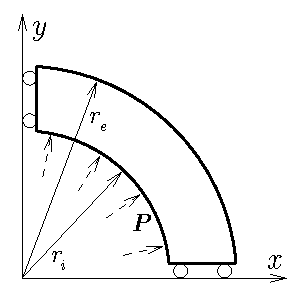
\includegraphics{cilipst}
\end{wrapfigure}
%\end{figure}


\end{document}
